\documentclass[a4paper, 12pt]{article}
\usepackage[margin=24mm]{geometry}
\usepackage{float}
\usepackage{titling}
\usepackage{graphicx}
\usepackage{caption}
\usepackage{subcaption}
\usepackage[hidelinks]{hyperref}
\usepackage[toc,page]{appendix}
\usepackage{multirow}
%
%\geometry{bindingoffset=35mm}

\providecommand{\keywords}[1]{\textbf{\textit{Keywords ---}} #1}

\begin{document}

\begin{titlepage}
\begin{center}{\LARGE
Electronics and Computer Science\\
Faculty of Physical and Applied Sciences\\
University of Southampton\\
\hfill \break
\hfill \break
\hfill \break\\
Merlin Webster\\
\today\\
\hfill \break
Skydiving Formation Recognition\\
\begin{figure}[H]
	\centering
	\includegraphics[width=.7\linewidth]{fs_silhouette.png}
\end{figure}
Project supervisor: Dr Jonathon S Hare\\
Second examiner: Prof Lie-Liang Yang\\
\hfill \break
\hfill \break
A project report submitted for the award of\\
MEng Electronic Engineering\\}
\end{center}
\end{titlepage}
%
\renewenvironment{abstract}
  {\small\quotation
  {\bfseries\noindent{\large\abstractname}\par\nobreak\smallskip}}
  {\endquotation}
%
\thispagestyle{empty}
\setcounter{page}{0}
\begin{abstract}\textbf{\emph{
Contrary to popular belief, skydiving is a competitive and technical sport, requiring careful control of body position in order to not only remain stable, but also to move around the sky in free-fall. A popular discipline in competitive skydiving is formation skydiving, where a group of skydivers form set shapes with their bodies whilst in free-fall. This Report proposes a software tool to be written; able to automatically judge  formation skydiving footage. This will be done detecting the pose of each skydiver in the formation individually; this information will then be used to find the overall shape of the formation. This tool will combine and extend well established computer vision methods such as Active Shape Models, skeletonisation. The ultimate goal is to remove the need for manual competition judging, switching to a fully automated system.
}}\end{abstract}
\keywords{computer vision, video analysis, formation skydiving, posture detection}
\clearpage

\textsc{\thispagestyle{empty}
\setcounter{page}{0}
\tableofcontents
\clearpage
\thispagestyle{empty}
\setcounter{page}{0}
\listoffigures 
\clearpage}

\section{Background}
	\subsection{Formation Skydiving}

		\subsubsection{Rules}

\section{Literature Report}

\section{System Design}

	\subsection{Flowchart}


\section{Project Management}

%
%
\clearpage
\begin{thebibliography}{9}
\bibitem{skeletonisation}
    Rafael C. Gonzalez \& Richard E. Woods,
    "Skeletons",
    Digital Image Processing -- Second Edition --- International Edition (2001),
    pg650-653
%
\bibitem{skeletonisation_simple}
    Rafael C. Gonzalez \& Richard E. Woods,
    "Skeletons",
    Digital Image Processing -- Second Edition --- International Edition (2001),
    pg543-545
%
\bibitem{binary_laplacian}
    Rafael C. Gonzalez \& Richard E. Woods,
    "The Laplacian",
    Digital Image Processing -- Second Edition --- International Edition (2001),
    pg581-585
%
\bibitem{Ramer}
    Urs Ramer,
    "An iterative procedure for the polygonal approximation of plane curves",
    Computer Graphics and Image Processing (1972),
    pg 244--–256
%
\bibitem{Douglas_Peucker}
	David Douglas \& Thomas Peucker,
	"Algorithms for the reduction of the number of points required to represent a 				digitized line or its caricature",
	The Canadian Cartographer (1973),
	pg112--–122
%
\bibitem{icl_pca}
	Imperial College London,
	"Lecture 15: Principal Component Analysis",
	\url{www.doc.ic.ac.uk/~dfg/ProbabilisticInference/IDAPILecture15.pdf},
	Last access: 9 Dec 2014
%
\bibitem{cootes}
	Tim Cootes, E. R. Baldock, \& J. Graham,
 	"An introduction to active shape models.",
 	Image Processing and Analysis(2000),
 	pg223---248
%
\bibitem{Piccardi}
	Piccardi, M., "Background subtraction techniques: a review," Systems,
	Man and Cybernetics,
	2004 IEEE International Conference,
	pg3099---3104 vol.4, 		
	(10-13 Oct 2004),
	doi: 10.1109/ICSMC.2004.1400815
%
\bibitem{OpenCV}
	OpenCV,
	"The OpenCV Reference Manual
	Release 2.4.9.0"(April 21, 2014),
	\url{http://docs.opencv.org/opencv2refman.pdf},
	Last access: 09 Dec 2014
%
\bibitem{Qt}
	Qt Project,
	"Qt Reference Pages",
	QtDoc 5.3,
	\url{http://docs.opencv.org/opencv2refman.pdf},
	Last access: 09 Dec 2014
%
\bibitem{2d_pose_detection}
	"Automatic Detection of 2D Human Postures Based
on Single Images",
	QtDoc 5.3,
	\url{http://docs.opencv.org/opencv2refman.pdf},
	Last access: 09 Dec 2014
%
\bibitem{monocular_still_images}
	Wachs, Juan P., Deborah Goshorn, and Mathias Kolsch,
	"Recognizing human postures and poses in monocular still images."(2009),
%
\bibitem{kinect_IR}
	Lu Xia, Chia-Chih Chen, Aggarwal, J.K.,
	"Human detection using depth information by Kinect,"
	Computer Vision and Pattern Recognition Workshops (CVPRW),
	2011 IEEE Computer Society Conference on , vol.,
	no., pp.15,22, 20-25 June 2011
doi: 10.1109/CVPRW.2011.5981811
%
\bibitem{video}
	Yu Tsz-Ho, Tae-Kyun Kim, and Roberto Cipolla,
	"Unconstrained monocular 3d human pose estimation by action detection and cross-			modality regression forest.",
	In Computer Vision and Pattern Recognition (CVPR),
	2013 IEEE Conference on, pp. 3642-3649. IEEE, 2013.
%
\bibitem{model-based}
Christophe Doignon (2007),
An Introduction to Model-Based Pose Estimation and 3-D Tracking Techniques,
Scene Reconstruction Pose Estimation and Tracking, Rustam Stolkin (Ed.), ISBN: 978-3-902613-06-6, InTech, pg360-376,
Available from:
\url{http://www.intechopen.com/books/scene_reconstruction_pose_estimation_and_tracking/an_introduction_to_m
odel-based_pose_estimation_and_3-d_tracking_techniques}
%
\bibitem{face_recognition}
Prabhu, Utsav, and Keshav Seshadri,
"Facial Recognition Using Active Shape Models, Local Patches and Support Vector Machines."
%
\end{thebibliography}
\clearpage
\begin{appendices}
%
\chapter{\textbf{A - Initial Gantt Chart}}
\label{appendix:a}
%
\begin{figure}[H]
	\centering
	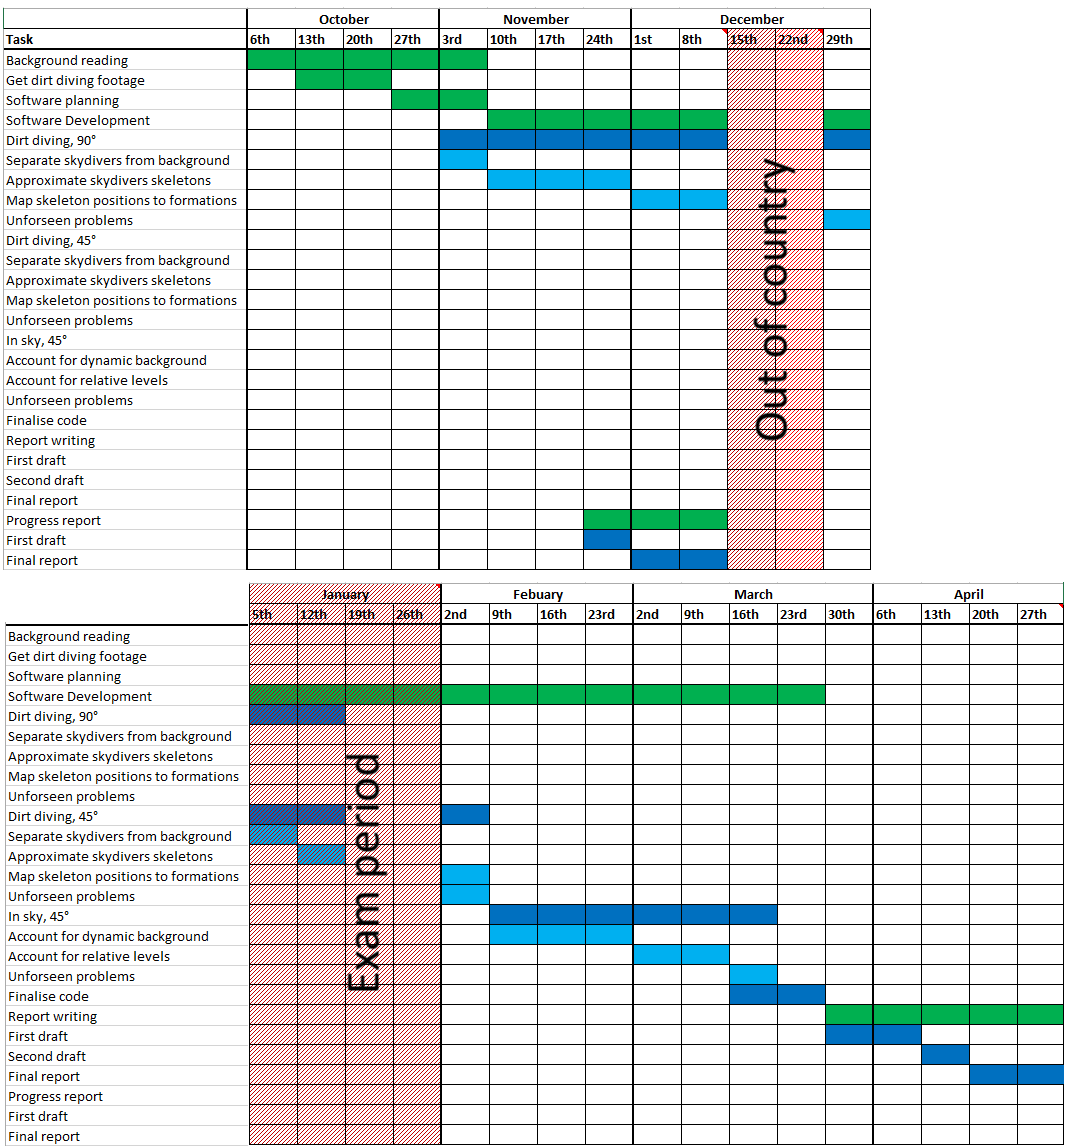
\includegraphics[width=\linewidth]{Gantt_initial_split.png}
	\caption{Initial Gantt Chart}
	\label{fig:gantt_initial}
\end{figure}
%
\chapter{\textbf{B - Revised Gantt Chart}}
\label{appendix:b}
%
\begin{figure}[H]
	\centering
	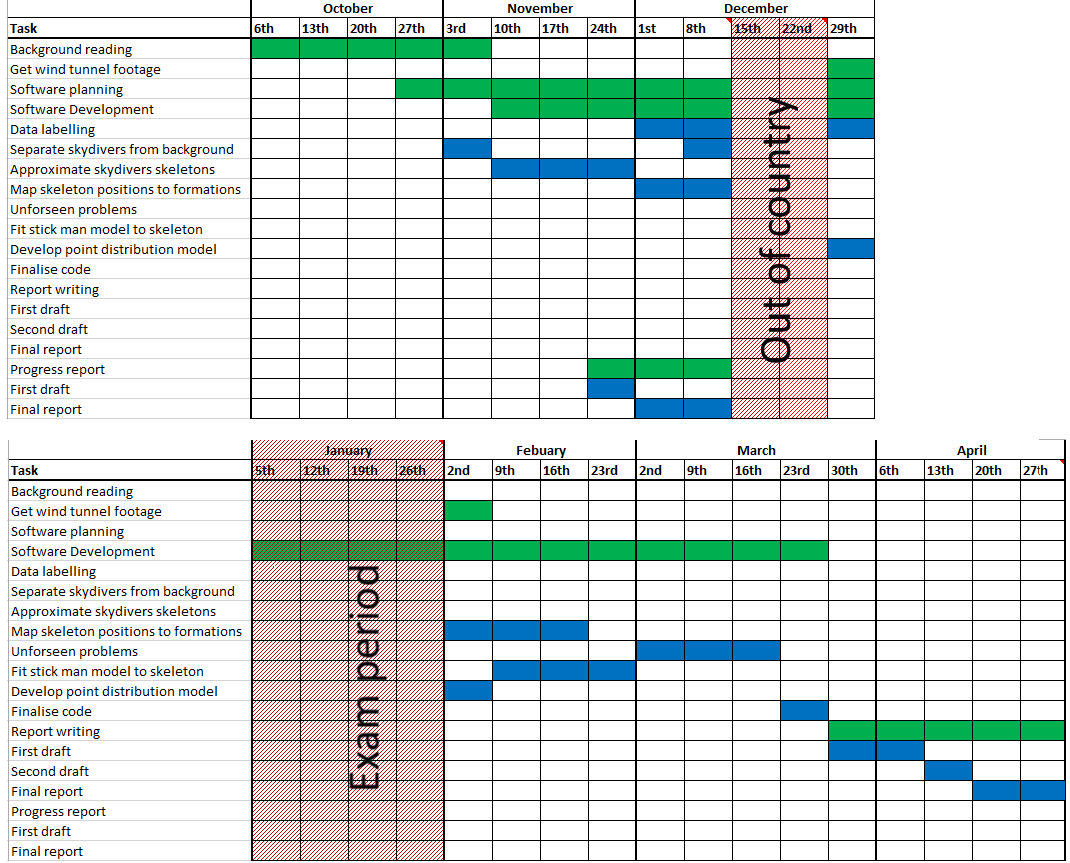
\includegraphics[width=\linewidth]{Gantt_new_split.png}
	\caption{Revised Gantt Chart}
	\label{fig:gantt_new}
\end{figure}
%
%
\end{appendices}
%
\end{document}